\documentclass{article}
\usepackage{main}

\title{Protocole TCP/IP}
\date{25 Septembre 2024}
\author{Seconde 9}

\begin{document}
\section*{Exemple de routage}
\begin{center}
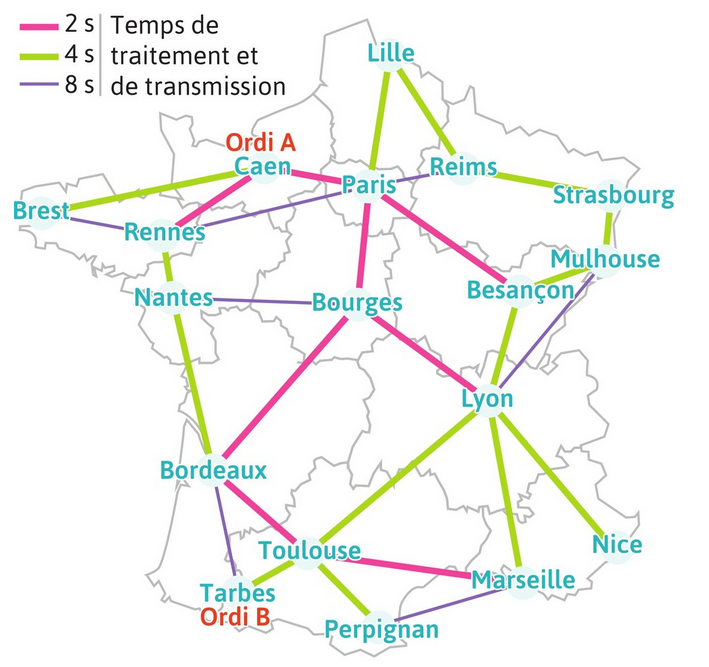
\includegraphics[width=0.9\textwidth]{Routage.png}
\end{center}

Chaque ville correspond ici à un routeur.

\begin{enumerate}[label=\emph{\alph*)}]
\item Décrire le routage le plus rapide pour transmettre un message de l'Ordi A vers l'Ordi B.

\emptybox{2cm}
\item Comme le routage est-il modifié si la connexion entre Paris et Bourges est coupée ?

\emptybox{2cm}
\item Du point de vue du routeur de Paris, vers quelle ville envoyer un message à destination de Marseille ? Et de Mulhouse ?

\emptybox{2cm}
\end{enumerate}
\end{document}
